\documentclass[12pt,a4paper]{article}

%\pdfoutput=1

\usepackage[utf8]{inputenc}
\usepackage[T1]{fontenc}
\usepackage[english]{babel}
\usepackage{amsmath}
\usepackage{mathabx}
\usepackage{lmodern}
\usepackage{dcolumn}
\usepackage{units}
\usepackage{siunitx}
\usepackage{icomma}
\usepackage{graphicx}
\usepackage{caption}
\usepackage{subcaption}
\usepackage{color}
\usepackage{pgf}
\DeclareMathOperator{\acosh}{arccosh}
\newcommand{\N}{\ensuremath{\mathbbm{N}}}
\newcommand{\Z}{\ensuremath{\mathbbm{Z}}}
\newcommand{\Q}{\ensuremath{\mathbbm{Q}}}
\newcommand{\R}{\ensuremath{\mathbbm{R}}}
\newcommand{\C}{\ensuremath{\mathbbm{C}}}
\newcommand{\rd}{\ensuremath{\mathrm{d}}}
\newcommand{\id}{\ensuremath{\,\rd}}
\usepackage{hyperref}
%\usepackage{a4wide} % puts the page numbering further down the page.
\usepackage{pdfpages}
\usepackage{epstopdf}
\DeclareGraphicsExtensions{.eps}

\title{Handin 2: Extraction of intrinsic parameters.}
\author{Marcus Malmquist, marmalm}
\date{\today}

\begin{document}
\maketitle

\section{Task 2}\label{sec:1}
In this section I describe the method I used to extract the values of intrinsic components. This method was proposed by Dambrine.
The simulation was set up according to Figure~\ref{fig:scematic}.
\begin{figure}
  \centering
  \noindent\makebox[\textwidth]{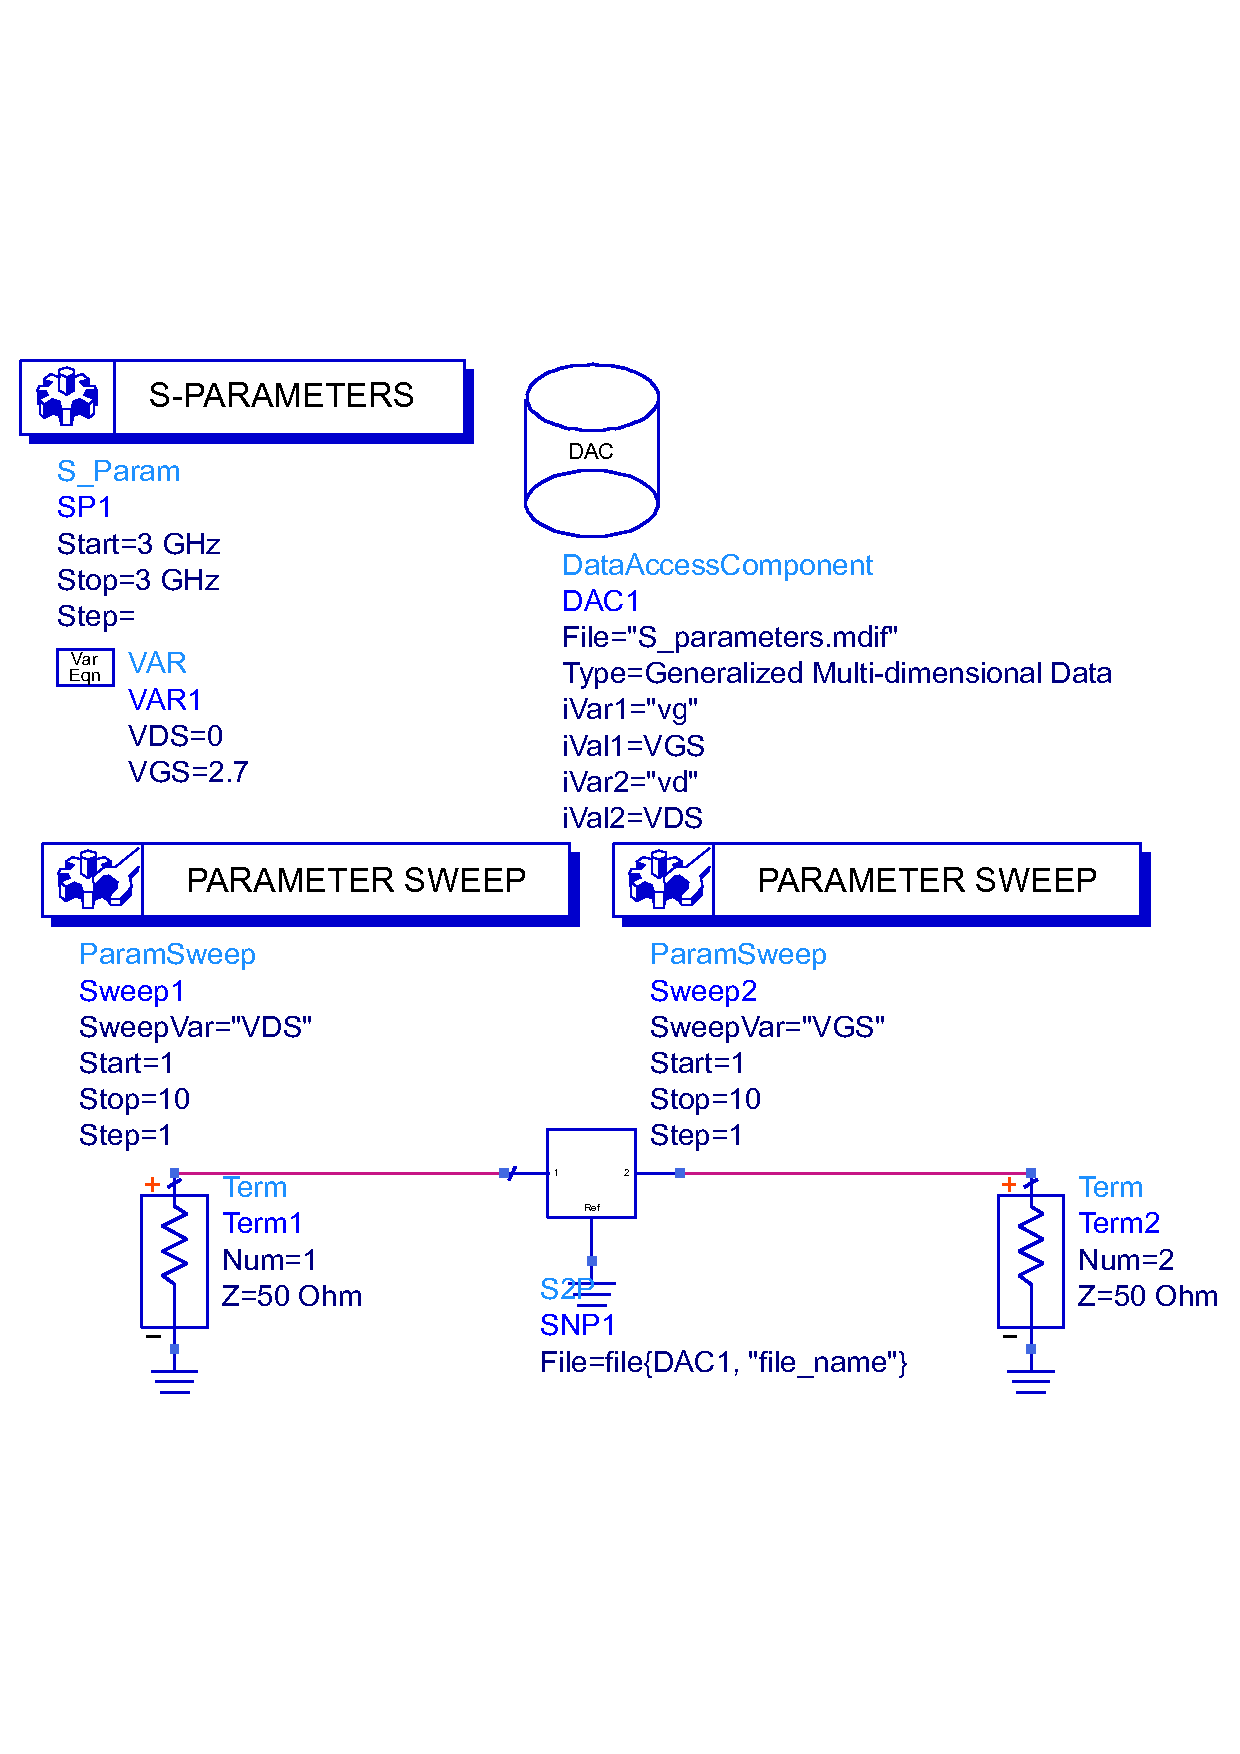
\includegraphics[width=\textwidth]{Task2_sc.pdf}}
  \caption{The scematic that was used to produce the results presented in this report.}
  \label{fig:scematic}
\end{figure}

Simulating the scematic shown in Figure~\ref{fig:scematic} yielded S-parameters for the two-port. The extrinsic parameters (calculated in the previous task) could be removed by a series of calculations.
\begin{itemize}
\item Convert $\mathbf{S}$ to $\mathbf{Y}_0$.
\item Remove extrinsic capacitances (\ref{eq:ex_c}).
\item Convert $\mathbf{Y}_1$ to $\mathbf{Z}_0$.
\item Remove extrinsic resistances and inductances (\ref{eq:ex_rl}).
\item Convert $\mathbf{Z}_1$ to $\mathbf{Y}$.
\end{itemize}
\begin{equation}
  \label{eq:ex_c}
  \mathbf{Y}_1 = \mathbf{Y}_0 -
  \begin{bmatrix}
    j\omega(C_\text{pg}-C_\text{pgd}) & -j\omega C_\text{pgd} \\
    -j\omega C_\text{pgd} & j\omega(C_\text{pg}-C_\text{pgd})
  \end{bmatrix}
\end{equation}
\begin{equation}
  \label{eq:ex_rl}
  \mathbf{Z}_1 = \mathbf{Z}_0 -
  \begin{bmatrix}
    R_g+R_s+j\omega(L_g+L_s) & R_s+j\omega L_s \\
    R_s+j\omega L_s & R_g+R_s+j\omega(L_g+L_s)
  \end{bmatrix}
\end{equation}
When the extrinsic parameters have been eliminated the intrinsic parameters can be acquired from (\ref{eq:in_param}), which yields seven equations (three real and four imaginary).
\begin{subequations}
  \label{eq:in_param}
  \begin{align}
    y_{11} &= R_iC_{gs}^2\omega^2+j\omega(C_{gs}+C_{gd}), \label{eq:in_param_y11}\\
    y_{12} &= -j\omega C_{gd}, \label{eq:in_param_y12}\\
    y_{21} &= g_m-j\omega\big(C_{gd}+g_m(R_iC_{gs}+\tau)\big), \label{eq:in_param_y21}\\
    y_{22} &= g_d+j\omega(C_{ds}+C_{gd}), \label{eq:in_param_y22}
  \end{align}
\end{subequations}
The intrinsic parameters can be seen in (\ref{eq:in_param_solve})
\begin{subequations}
  \label{eq:in_param_solve}
  \begin{align}
    R_j &= -\Re\Big(\frac{1}{y_{12}}\Big), \label{eq:in_param_solve_rj}\\
    C_{gd} &= \frac{1}{\omega\Im\big(\frac{1}{y_{12}}\big)}, \label{eq:in_param_solve_cgd}\\
    R_i &= \Re\Big(\frac{1}{y_{11}+y_{12}}\Big), \label{eq:in_param_solve_ri}\\
    C_{gs} &= -\frac{1}{\omega\Im\big(\frac{1}{y_{11}+y_{12}}\big)}, \label{eq:in_param_solve_cgs}\\
    R_{ds} &= \frac{1}{\Re(y_{12}+y_{22})}, \label{eq:in_param_solve_rds}\\
    C_{ds} &= \frac{\Im(y_{12}+yielded_{22})}{\omega}, \label{eq:in_param_solve_cds}\\
    g_m &= \Bigg|\frac{(y_{12}-y_{21})(y_{11}+y_{12})}{\Im(y_{11}+y_{12})}\Bigg|, \label{eq:in_param_solve_gm}\\
    \tau &= \frac{\frac{\pi}{2}-\angle(y_{12}-y_{21})+\angle(y_{11}+y_{12})}{\omega} \label{eq:in_param_solve_tau}
  \end{align}
\end{subequations}
Using the extrinsic parameters calculated during the previous handin yields the values in Table~\ref{tab:in_vals}
\begin{table}
  \centering
  \begin{tabular}{|l|r|}\hline
    Variable & Value \\ \hline
    $R_j$ & $\SI{2.28}{\kilo\ohm}$ \\
    $C_{gd}$ & $\SI{-23.3}{\femto\farad}$ \\
    $R_i$ & $\SI{5.38}{\ohm}$ \\
    $C_{gs}$ & $\SI{-57.3}{\femto\farad}$ \\
    $R_{ds}$ & $\SI{-7.58}{\kilo\ohm}$ \\
    $C_{ds}$ & $\SI{-208}{\femto\farad}$ \\
    $g_m$ & $\SI{2.30}{\milli\siemens}$ \\
    $\tau$ & $\SI{88.3}{\pico\second}$ \\ \hline
  \end{tabular}
  \caption{The final values of the intrinsic parameters.}
  \label{tab:in_vals}
\end{table}

The calculations were done in ADS and the procedure can be seen in Figure~\ref{fig:calcs}.
\begin{figure}
  \centering
  \noindent\makebox[\textwidth]{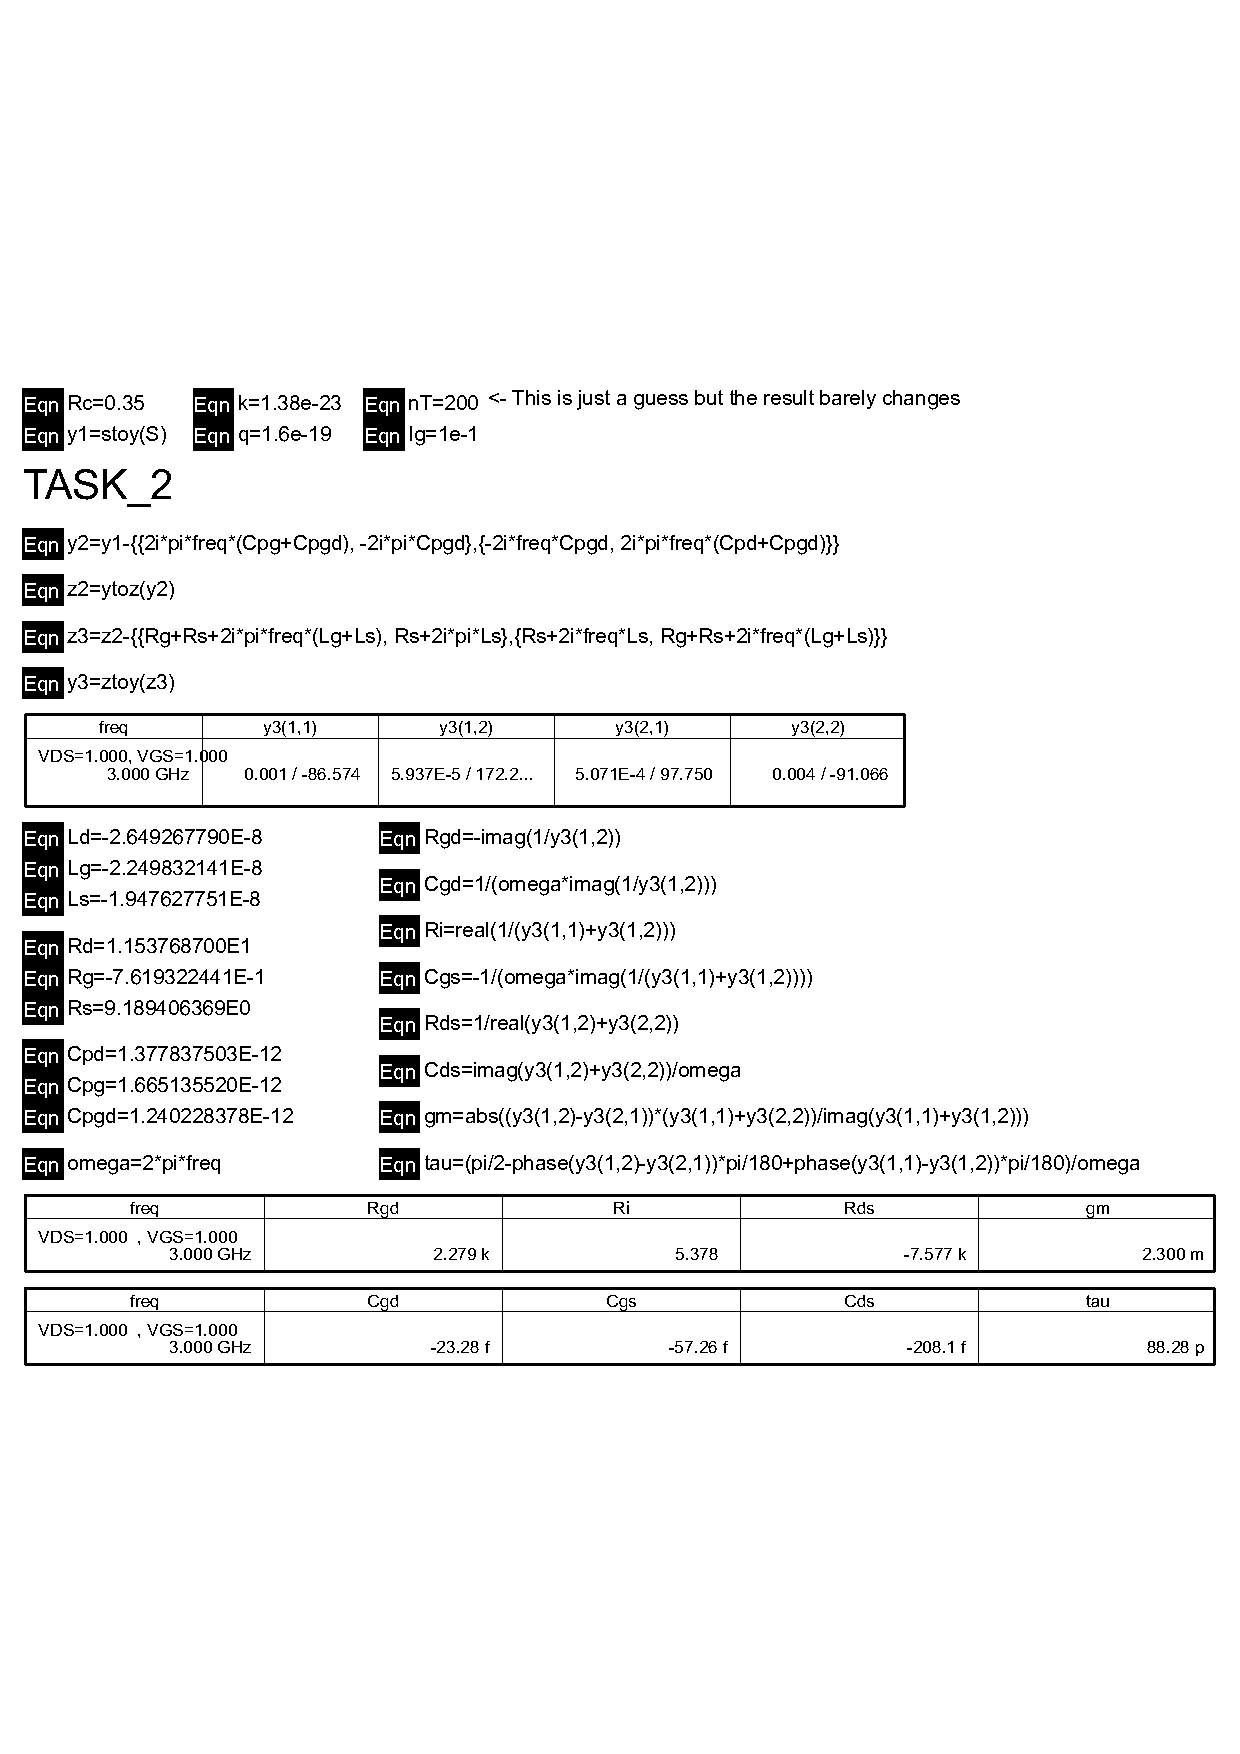
\includegraphics[width=\textwidth]{Task2.pdf}}
  \caption{The cell that was used to produce the results presented in this report.}
  \label{fig:calcs}
\end{figure}

\end{document}